\chapter{Gold nanorods as nano-thermometers}
\label{ch:AntiStokes}

\begin{abstract}
Nano-thermometry is a challenging field that can open the door to very
intriguing results ranging from biology and medicine to material sciences. Gold
nanorods are excellent candidates to act as nanoprobes because they are
efficient light emitters upon excitation with a monochromatic source. Moreover
gold nanoparticles are already used in photothermal therapy as efficient
transducers of electromagnetic radiation into heat. In this work we show that
the spectrum of the anti-Stokes emission from gold nanorods irradiated in
resonance can be used to measure the absolute temperature of the nanoparticles.
The procedure does not require any previous calibration and can be easily
implemented in any microscope capable of acquiring emission spectra. We show
that the luminescence spectrum of single gold nanorods closely follows
Bose-Einstein statistics. We model the emission considering interactions of the
electrons and holes created upon absorption of a photon with phonons in the
metal.
\end{abstract}

\newpage

\section{Introduction}
\dropcap{M}{ost} physical, chemical, biological processes depend on temperature.
Together with the miniaturization of devices and the advent of nanotechnology the need
for measuring temperature with high spatial accuracy started to emerge. Notably
in biology\cite{Yang2011a,Hrelescu2010} and medicine\cite{Li2013c} measuring and
controlling temperature at a single cell level will provide not only insight
into intracellular processes but it will also contribute to a better
understanding of the mechanisms involved in the proposed new therapies such as
photothermal tumor ablation\cite{Gobin2007} or controlled drug
delivery\cite{Huang2006,Huo2014}. 

Probes with distinctive spectral features are ideal candidates for temperature
measurements since they provide high spatial accuracy while far field optics
allow a non-contact readout. Some of the proposed strategies include structures
that undergo a conformational change upon an increase in
temperature\cite{Ebrahimi2014}, thus inducing variations in fluorescence
intensity of a dye molecule embedded into them. Also cleverly designed
fluorescent probes\cite{Vetrone2010} in which the ratio of particular emission
peaks depends on temperature allow a high accuracy and can be used for
intracellular thermometry.

The use of anti-Stokes fluorescence emission from lanthanide ions has been
studied for several years\cite{Auzel2004a} and can be used to determine
temperature with high accuracy. However organic dyes show a very low amount of
emitted photons with a higher energy than the excitation energy, rendering their
use in biological conditions very challenging. Recently Surface Enhanced Raman
Spectroscopy (SERS) allowed to measure changes induced by temperature down
to single molecules\cite{Pozzi2015}, but a careful calibration of the
measurements is crucial.

At a cellular level measuring temperature has been subject to extensive
debates\cite{Yang2011a,Suzuki2015}. Many cellular processes may be subject to
temperature variations, including heat generation at mitochondria. However the
measured temperatures\cite{Yang2011a} are in the order of $10^5$ times higher
than the expected values drawn from theoretical models\cite{Sato2014}.
Moreover new applications in photothermal therapy require locally increasing the
temperature in order to induce the death of specific cells in a
tissue\cite{Huang2008,Huang2006}. Many of these methods employ metallic
nanoparticles as heat sources\cite{Gobin2007,Hirsch2003} but rely on
models\cite{Zhao2014a} or on ad-hoc calibrations to estimate the temperatures
reached\cite{Donner2013}. Therefore a method that allows both to increase the
local temperature and to monitor it will be of great interest in a broad range
of fields.

Gold nanoparticles continue to receive a great amount of attention because of
their unique optical properties\cite{Zijlstra2011}. The collective oscillation
of conduction electrons, also known as plasmon, shows a resonance in the visible to
near infra-red wavelengths. This resonance can be tuned by changing the shape of
the particles\cite{Carattino2016} and will be responsible for a large absorption
and scattering cross section at the resonance wavelength. It is therefore simple
to detect nanoparticles in a dark field scattering\cite{Hu2008} configuration or
via photothermal imaging\cite{Berciaud2006}. Detecting the particles through
their luminescence\cite{Tcherniak2011} is also possible; their low quantum
yield\cite{Fang2012,Rao2015,Yorulmaz2012,Cheng2015}, in the order of $10^{-5}$
is compensated by the enhanced cross section. Moreover the luminescence signal
is stable over time; gold nanoparticles do not blink nor bleach, therefore are 
useful labelling agents for processes that require extended periods of
observation\cite{Wang2005}.

Different metallic nano-objects are being introduced as agents for photothermal
therapy or drug delivery\cite{Kang2013}. One of the advantages of gold
nanoparticles is the possibility of tuning their resonance to the near infra-red
range, where the penetration of light into tissues can be of several
centimeters\cite{Huang2006,Gobin2007,Hirsch2003,ONeal2004,Li2013c,Huang2008}.
Moreover the particles can be used not only for treatment, but also for
imaging\cite{Zhao2014a,Huang2006}. In this work we propose that the anti-Stokes
luminescence of gold nanorods and nanospheres can be used to measure their
temperature with relatively high accuracy.

Luminescence of metallic nanoparticles has been the object of extensive study in
recent years. Since the first observation of luminescence from bulk
gold\cite{Mooradian1969}, different groups have tried to quantitatively describe
the observed properties\cite{Mohamed2000,Beversluis2003a}, such as the quantum
yield\cite{Fang2012,Rao2015,Yorulmaz2012,Cheng2015,Dulkeith2004} and the
emission spectrum\cite{Link2010}. Several computer
packages\cite{Yurkin2011,Draine1994,Oskooi2010} allow to calculate the cross
sections of different geometries and there are already several successful
applications of nanoparticles into different
fields\cite{Fedoruk2013,Huang2006,Huang2008,Zijlstra2009}.  

Luminescence from single gold nanoparticles can be observed when
irradiating them with a monochromatic source. Gold nanorods present two distinct
resonance energies, namely the transverse and the longitudinal plasmon
resonance. These particles can therefore be excited efficiently at one of those
energies; the transverse resonance corresponds to a wavelength of $532\nm$ and will give
rise to a broad emission with a peak at the longitudinal plasmon energy.
Conversely it is possible to excite the particles with a wavelength matching
the longitudinal plasmon resonance. In this case the excitation benefits from
an enhanced absorption cross section, but the emission that overlaps the plasmon
resonance will be mostly blocked by the filters needed to prevent direct
excitation light from reaching the detectors.

In this work luminescence refers to the emission from nanoparticles observed at
energies different from the excitation energy. Normally it is expected that
after absorption of a photon, the electrons in the particle will relax and the
emitted photon will appear at lower energies than the excitation. If this is the
case, the emission is called Stokes-shifted; however gold nanoparticles when
excited in resonance also present a significant emission at higher energies.
This anti-Stokes emission from nanorods has been largely overlooked in
previous literature. Its characterization is the cornerstone of this work.

The mechanism we propose to explain the luminescence from gold nanoparticles is
based on the radiative recombination of electron and holes that are created upon
the absorption of an incident photon\cite{Dulkeith2004,Mooradian1969}. The
emission will be enhanced by the presence of the surface plasmon acting as an
antenna\cite{Mohamed2000}. At the same time, the probability of the interaction
of the electron or hole with a thermal bath (a phonon or a carrier) before
recombining can give rise to an emitted photon with a higher energy than the
excitation\cite{Hodak2000,Giri2015,Arbouet2003a}.

A monochromatic photon with energy $\hbar\omega_\textrm{L}$ incident on the
particle will give rise to a collective oscillation of the gas of conduction
electrons called plasmon. The lifetime of the oscillation can be measured in
pulsed experiments or calculated from the inverse of the linewidth and is in the
order of $10\fs$\cite{Sonnichsen2002}. The plasmon decays by forming a pair of
hot electron and hole with an energy difference equal to the plasmon
energy\cite{Sundararaman2014,Brongersma2015,AlejandroManjavacasJunG.LiuVikramKulkarni2014}.

The hot electron and hole cool down by exchanging energy with the lattice on a
timescale of $\tau\approx1\ps$\cite{Pustovalov2005}. Before this happens,
electron and hole have a small probability of recombining radiatively, i.e. of 
re-emitting their high electronic energy as a photoluminescence photon. If they
have interacted only with static surfaces, their energy would be the same and
therefore the emitted photon would have the same energy as the incoming
photon, and will not contribute to the measured photoluminescence (as it will be
blocked by the notch filter.) If on the other hand they have interacted with a
phonon or a thermally excited electron or hole, they may have lost or acquired
energy before recombining.

Electron and hole can also interact with baths upon recombination, either by
creation or annihilaton of a phonon. In both cases the energy available upon
recombination cannot much exceed $\hbar\omega_L+k_BT$. It has to be noted that
in the hypothesis of a single-photon absorption at low excitation power, the
temperature $T$ is that of the baths before absorption, i.e. the temperature of
the medium surrounding the particle. This is different from pulsed experiments,
in which the electron gas temperature can be orders of magnitude higher than
room temperature\cite{Baffou2013a}. 

Radiative recombination gives rise to weakly emitting sources spectrally adn
spatially distributed throughout the particle over a broad frequency band with
an exponential cutoff at $\hbar\omega_\textrm{L}+k_\textrm{B}T$. The weak
recombination emission can be greatly enhanced by the surface plasmon resonance,
acting as an antenna. With this model the following predictions can be made.
Firstly the emission spectrum must follow the plasmon spectrum if the excitation
laser is well above the plasmon resonance as shown in \mbox{Figure
\ref{fig:spectra_rod}} in the results. If the excitation falls within the
plasmon resonance, the spectrum is expected to follow the plasmon spectrum
multiplied by Bose-Einstein statistics factor arising from phonon population.
This factor should be proportional to $\bar{n}$ for anti-Stokes and $\bar{n}+1$
for Stokes processes, where

\begin{equation}
	\bar{n}=\left(\exp\frac{\hbar\omega}{k_bT}-1\right)^{-1}.
\end{equation}

With this model, it can also be predicted that the emission should be polarized;
for the longitudinal plasmon of gold nanorods this polarization coincides with
the longitudinal axis of the particle\cite{He2015}. Moreover, the lifetime
should be determined by the lifetime of hot electrons and holes and should be
significantly shorter than the thermalization time of the carriers. If this was
not the case, some interactions would be enough to reduce the carriers' energy
and therefore the electron and hole wouldn't have enough energy to produce an
optical photon. Finally only the presence of hot carriers is required in the
model. As the wavevectors are randomly distributed at all times, the
recombination probability remains constant at all stages of relaxation.
Therefore excitation well above the plasmon resonance should excite the
photoluminescence with nearly the same efficiency as just above the plasmon
resonance\cite{Cheng2015}. Differences in the distribution of electron and holes
appear if the excitation energy allows interband
transitions\cite{Sundararaman2014,Brown2016}. These transitions are more
sensitive to the band structure of the material than intraband transitions,
where electrons can be treated as free particles in a potential. 

In this work we propose to use the anti-Stokes luminescence emission from gold
nanoparticles to determine their temperature. According to the model just
described, the anti-Stokes emission follows the following form,

\begin{equation}\label{eqn:fitting}
	I(\omega) =
	\textrm{I}_{\textrm{SPR}}(\omega)\cdot\left(\exp\frac{\hbar(\omega-\omega_\textrm{L})}{k_\textrm{B}T}-1\right)^{-1}
\end{equation}

\noindent where $I$ is the intensity, $\omega$ is the angular frequency of the
photons, $\omega_\textrm{L}$ is the frequency of the laser, $\hbar$ is Planck's
constant, $k_\textrm{B}$ the Boltzmann constant. $\textrm{I}_{\textrm{SPR}}$ is
the photo luminescence spectrum of the surface plasmon resonance that can be
obtained by exciting the particle at energies higher than the resonance, or by
looking at the scattering spectrum. The only remaining free parameter is the
temperature $T$ (plus a normalization constant not included in eqn.
\ref{eqn:fitting}.) This means that carefully fitting the emission spectra
excited at two frequencies ($\nu\gg\nu_{\textrm{SPR}}$ and
$\nu\approx\nu_{\textrm{SPR}}$) allows us to extract the absolute temperature of
the particles without any previous calibration.


\section{Experimental method}
All the measurements in this work were performed with a home-built confocal
microscope equipped with an APD and a spectrometer (Acton 500i). Samples were
mounted in a flow cell that allowed us to increase the temperature of the medium
up to $60\,^oC$ and to monitor it through a Pt100 resistance thermometer placed
$1\mm$ away from the observation area.

Samples were prepared by spin casting a suspension of nanoparticles onto clean
coverslips. Different particles were employed in this work. Nanorods with
average dimensions of $21\nm\times50\nm$ and a plasmon resonance around $650\nm$
were synthesized following the seeded-growth method\cite{Nikoobakht2003};
spheres with radii between $30\nm$ and $60\nm$ were purchased from BBI
International. We employed a $532\nm$ (CNI) laser for characterizing the
nanorods' plasmon and for exciting spheres close to resonance. A $633\nm$ HeNe
(Thorlabs) was employed to excite the nanorods in resonance.

Room temperature measurements were performed using a $60X$, NA $1.4$ oil
immersion objective (Olympus). This provided high excitation and collection
efficiency. At higher temperatures an air-spaced objective, $60X$, NA $0.9$
(Olympus) was employed to avoid the presence of a heat sink directly in contact
to the observed area. With this objective both the excitation and collection
efficiencies are significantly lower. The lower excitation efficiency can be
compensated increasing the excitation power, the lower collection however is
inherent to the method and can be compensated only by increasing the exposure
time.

To compensate for the drift of the setup while increasing the temperature, we
developed a computer program to continuously track a reference particle. The
same program was responsible for recording the temperature and triggering the
spectrometer. In this way complete data sets were acquired at different
temperatures, including spectra while exciting at $532\nm$, at $633\nm$ with
different laser intensities and the temperature measured by the Pt100. A
spectrum with $532\nm$ laser excitation was taken after every cycle to ensure
that the particle was not reshaping due to higher excitation powers.

The intensity of the lasers was controlled via the voltage applied to an AOM in
the optical path. Several accumulations of the spectra at the same laser
intensity were recorded. This not only allowed us to lower the noise of the
measurements because of a longer exposure time, but also allowed us to remove
bright pixels generated by cosmic rays. Having several accumulations is also
useful to monitor changes in the intensity of the spectra during the acquisition
itself. These changes can be due to a drift of the setup while measuring or to a
reshaping of the particle. The reshaping can be confirmed by comparing the
spectra acquired with the $532\nm$ laser\cite{Liu2009} and in that case the
measurements where not considered. In the case of drift of the setup, the
particular data set was not taken into account. For the purposes of this
work the excitation intensity is crucial for characterizing the method;
if the particle is not in focus it would result in an over estimation of the
excitation power. 

To calculate the heating of the particles the absorption cross section has to be
computed. For the case of nanorods, the ADDA package was
employed\cite{Yurkin2011}. Spheres' cross section can be calculated from Mie
theory. Once the dissipated power is known, the parameters can be either used in
a Comsol model or the heat equation can be analytically solved, approximating
the rods by spheres with the same total area.

\section{Results}
\begin{figure}[htp] \centering
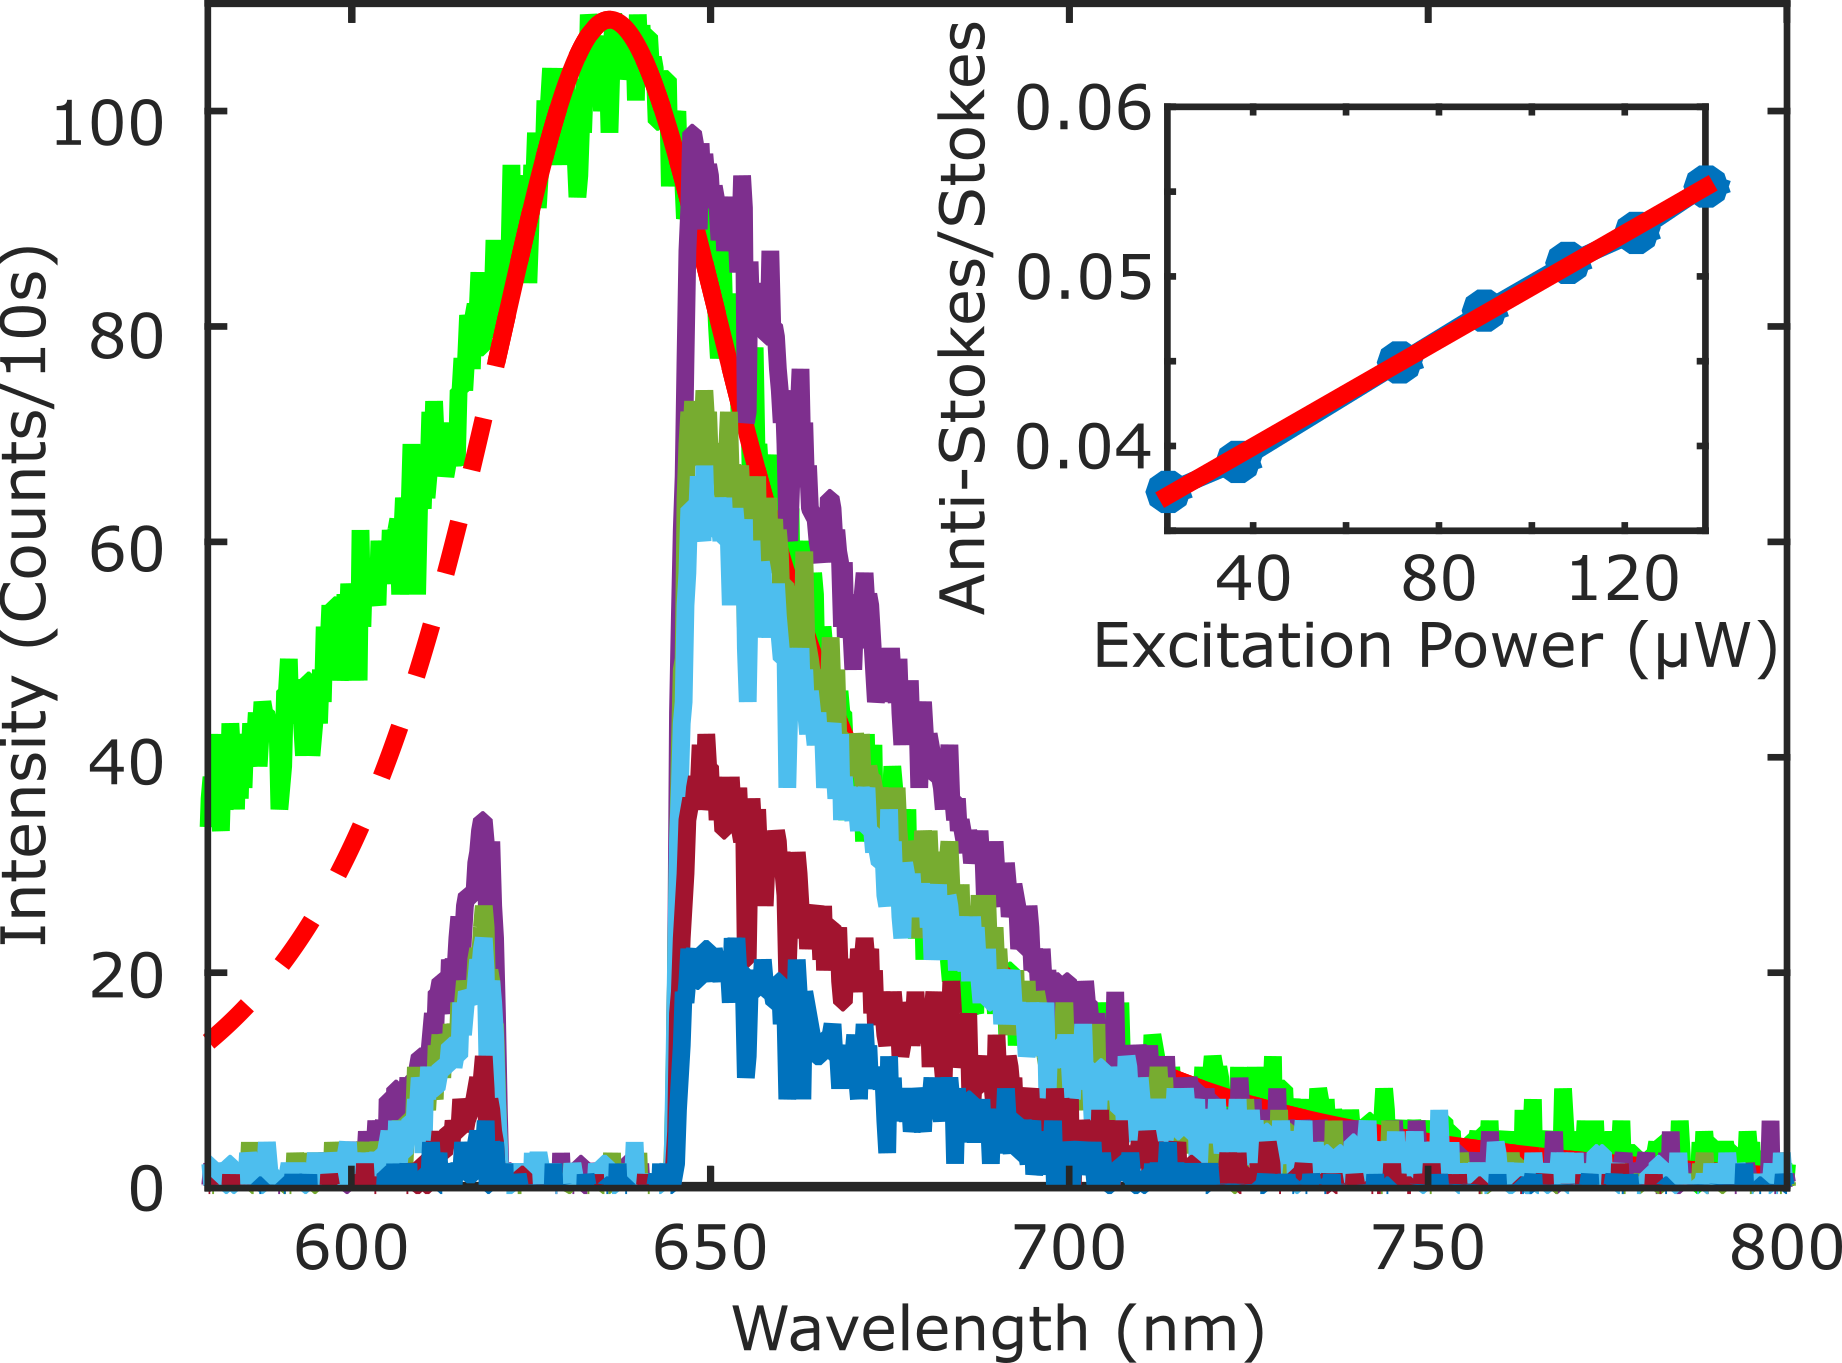
\includegraphics[width=0.45\textwidth]{Chapters/04_Anti-Stokes/Figures/02_Several_Intensities/02_several_intensities.png}
\caption{Luminescence spectra of a single gold nanorod. The green curve is the
emission under $532\nm$ excitation. In red is the fitting by a lorentzian; the
dashed part is the region that was not considered for the fitting. The other
curves are the emission of the same particle under $633\nm$ irradiation at three 
different powers. The inset shows the anti-Stokes-to-Stokes ratio as a function
of the excitation power, overlapped with a linear fit in red.}
	\label{fig:spectra_rod}
\end{figure}

The proposed model for the anti-Stokes emission requires to know the plasmon
spectrum ($\textrm{I}_{\textrm{SPR}}$ function in equation \ref{eqn:fitting}) of
the particle in order to fit the emission at shorter wavelengths and extract the
particle temperature. It has been shown that both scattering and luminescence
spectra roughly overlap over a broad range of wavelengths\cite{Yorulmaz2012}. Therefore
exciting gold nanorods with $532\nm$ allows to record the longitudinal plasmon
spectra, as shown in the green solid curve of Figure \ref{fig:spectra_rod}. The
peak was fitted by a single lorentzian, shown in red in the Figure; the dashed
part of the curve depicts the spectral region that was not considered for the
fitting. It has to be recalled that the luminescence spectrum is not a perfect
lorentzian since there is a broadband contribution to the luminescence arising
between the excitation wavelength and the plasmon peak\cite{Boyd1986}. This
appears as an asymmetry in the emission spectrum, particularly visible for
wavelengths smaller than $625\nm$. The results of this fitting will be employed
for the SPR function defined in equation \ref{eqn:fitting}. A lengthier
discussion on the effects of this procedure is given in the Supporting
Information.

The other curves in Fig. \ref{fig:spectra_rod} show the luminescence emission of
the same nanorod while irradiating with a $633\nm$ laser at different powers,
ranging from $25\uW$ to $75\uW$ at the back aperture of the objective. The
vertical black line shows the wavelength of the laser. The Stokes part of the
spectrum at longer wavelengths than the excitation shows the same shape as the
plasmon emission observed under $532\nm$ excitation, apart from a normalization
factor. From the figure it can readily be seen that the shape of the anti-Stokes
emission, at shorter wavelengths than excitation, is exponential-like and
doesn't follow the lorentzian shape of the Stokes emission. The dip between
Stokes and anti-Stokes is caused by the notch filter that prevents direct
excitation light from reaching the detectors.

The inset of Fig. \ref{fig:spectra_rod} shows the anti-Stokes-to-Stokes ratio of
the integrated luminescence for different laser excitation intensities. It is
possible to see that even with a linear behavior, the anti-Stokes intensity
increases more rapidly with laser excitation power than the Stokes emission.
We already exploited this phenomenon to image gold nanorods in high-background
conditions\cite{Carattino2016a}. Moreover it shows that the anti-Stokes emission
depends on laser excitation power differently from its Stokes counterpart. 

Figure \ref{fig:Log_Plot} shows the intensity of the Stokes (red) and
anti-Stokes (blue) emission for several excitation powers. In both cases the
linear fit in logarithmic scale has a slope close to $1$, being $0.88$ for the
Stokes and $1.20$ for the anti-Stokes, confirming that both types of emission
are single-photon processes. The behavior is independent of the plasmon
resonance position. It is important to note that the excitation intensity cannot
be increased much beyond what is shown because nanorods would start reshaping
towards a more spherical shape at higher laser powers.

\begin{figure}[htp] \centering
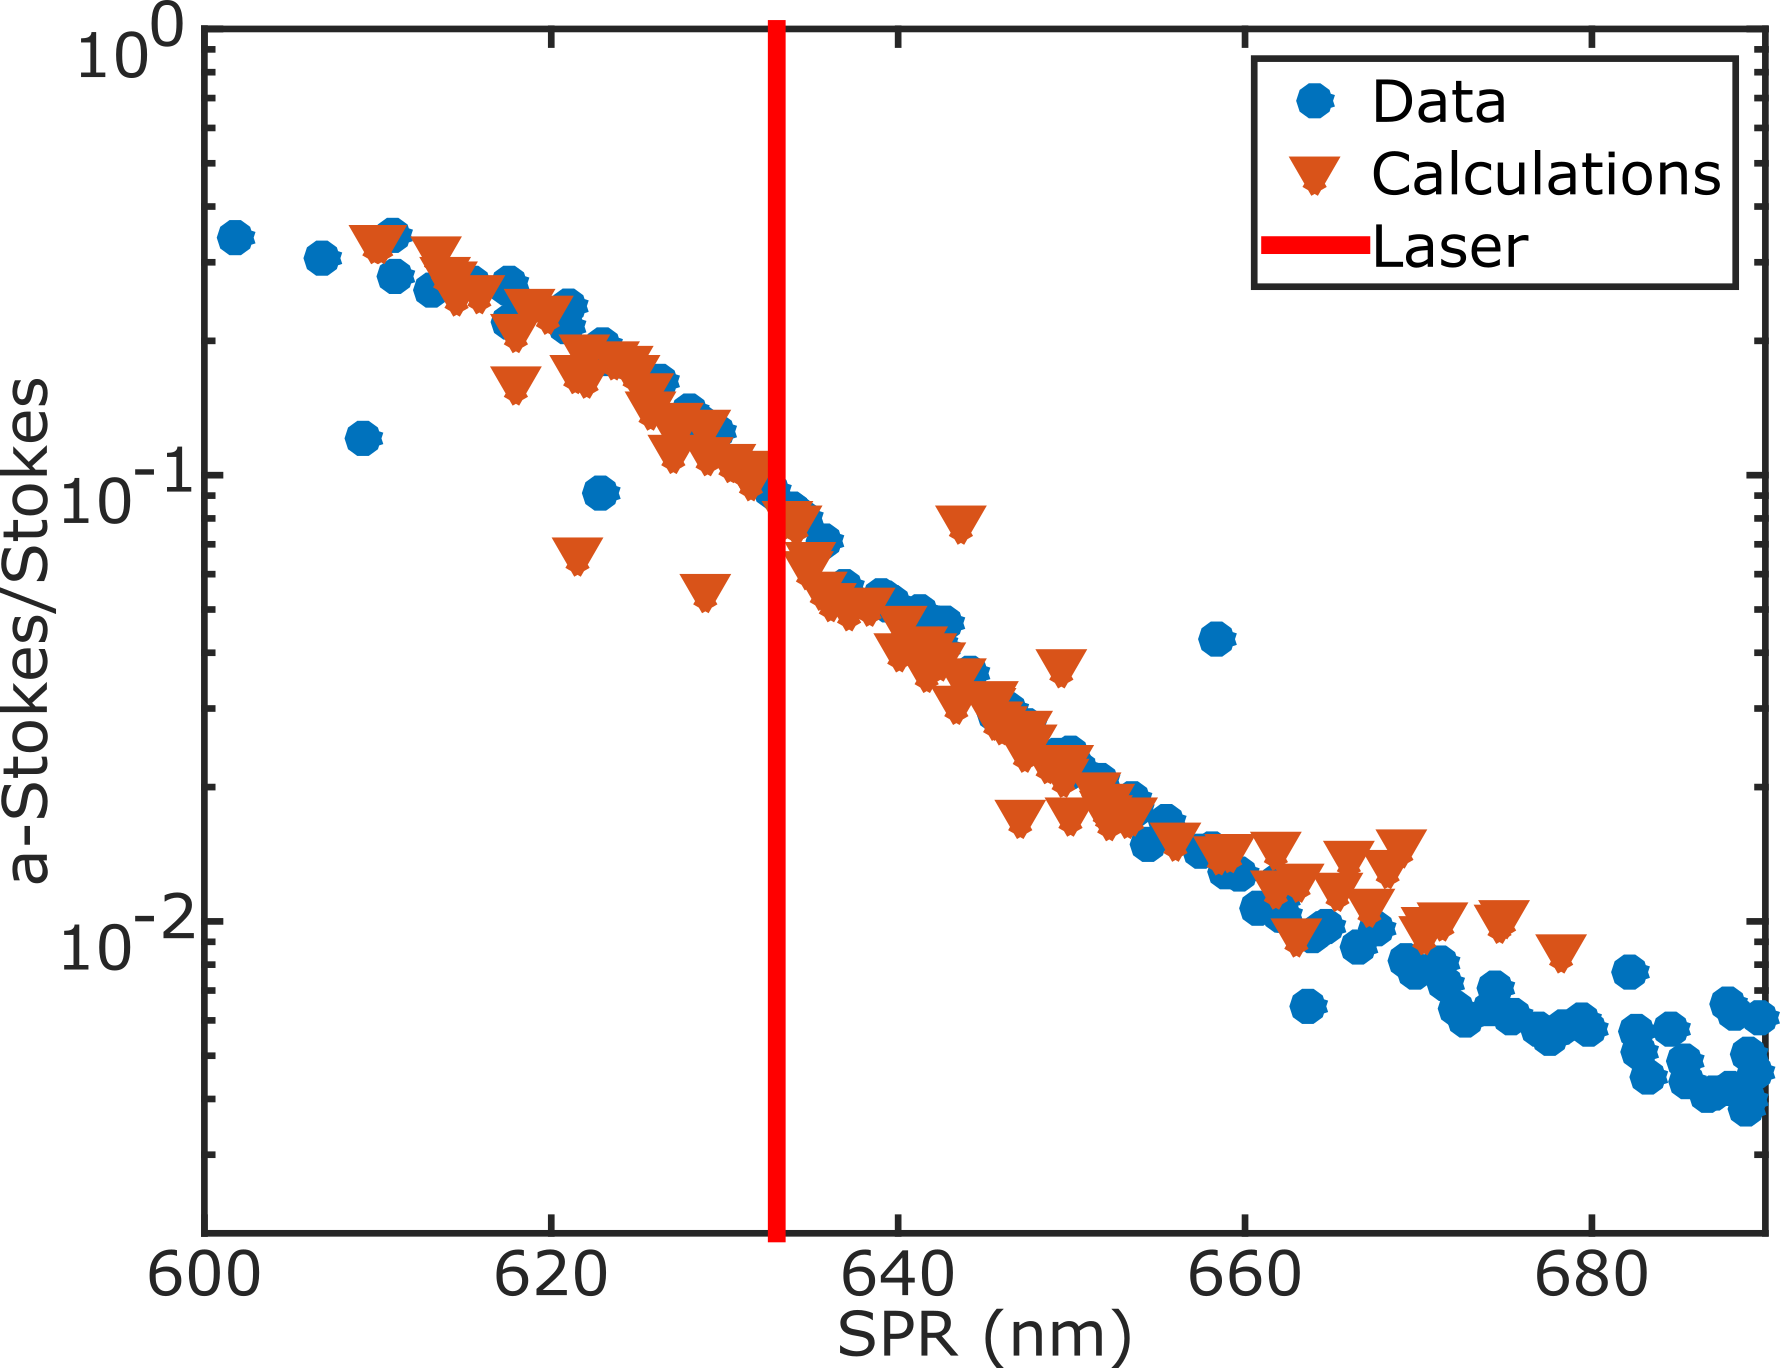
\includegraphics[width=0.45\textwidth]{Chapters/04_Anti-Stokes/Figures/Supplementary/02_AS_vs_S_SPR/02_AS_vs_S_SPR.png}
\caption{Ratio of the anti-Stokes to Stokes emission under $633\nm$
excitation as function of the resonance wavelength of each particle.
The blue circles are experimental results, while the red triangles are
the results of the calculations with equation \ref{eqn:antiStokes}. There is a
very good agreement between experiment and calculations. Particles with a
resonance to the blue of the laser (vertical red line) have an increase in the
anti-Stokes emission.}
	\label{fig:ASS-ratio}
\end{figure}

Figure \ref{fig:ASS-ratio} shows the ratio of the anti-Stokes to Stokes emission
for $90$ nanorods with different plasmon resonances and under $633\nm$
excitation; the blue circles are experimental data. The horizontal axis of the
figure is the surface plasmon resonance (SPR) of each particle. The vertical red
line marks the laser wavelength. The particles shown in the plot had resonances
between $600\nm$ and $690\nm$; the ones showing the maximum ratio of anti-Stokes
to Stokes are those with a resonance to the blue of the laser. For these
particles the plasmon is enhancing preferably the anti-Stokes emission. For
particles with a resonance at the laser wavelength the anti-Stokes and the
Stokes emission have similar enhancement and show a ratio close to $10\%$. 

Figure \ref{fig:ASS-ratio} also shows the results of calculations as the red
triangles. A very good overlap between the measured and the calculated data can
be observed. The absorption cross section of several particles was calculated
with the ADDA package. Each calculated absorption spectrum was fitted by a
lorentzian and used as $\textrm{I}_{\textrm{SPR}}(\omega)$ in eqn.
\ref{eqn:fitting}. The absorption cross section also allowed us to estimate the
temperature of the particle assuming a diffraction limited laser spot and from
this to calculate the emission spectrum of the anti-Stokes using the full eqn.
\ref{eqn:fitting}. The Stokes emission was calculated assuming a lorentzian
spectrum overlapping the absorption cross section. Both anti-Stokes and Stokes
emissions are proportional to the excitation power, but this term cancels out
when computing the ratio. For this calculation no free parameters were assumed
and the transmission of the filters was taken into account.

\begin{figure}[htp] \centering
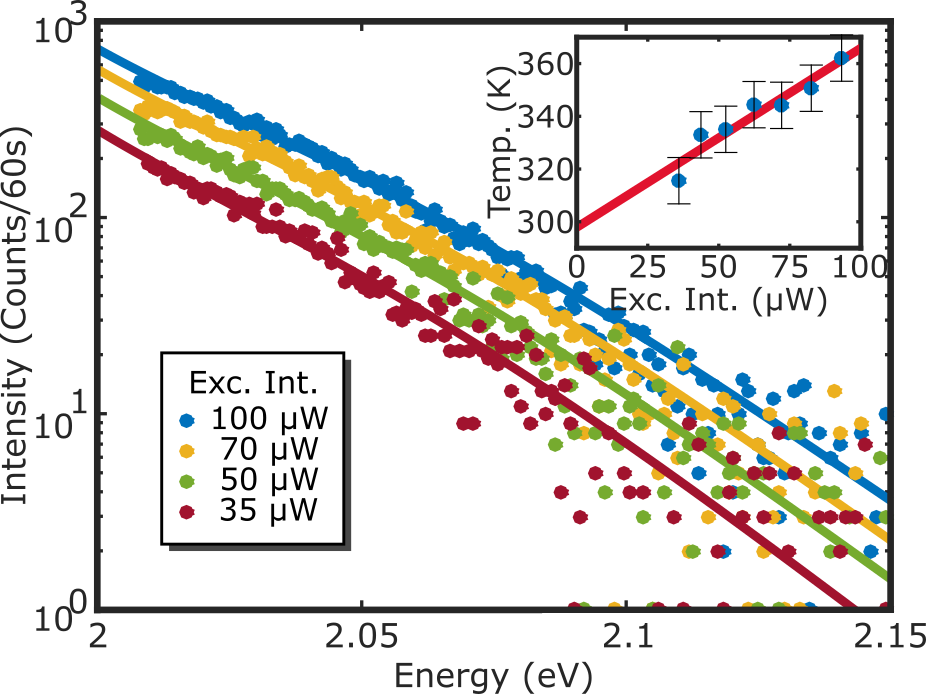
\includegraphics[width=\textwidth]{Chapters/04_Anti-Stokes/Figures/03_Fit_Of_AS/03_Log_Fit_AS.png}
\caption{a) Anti-Stokes emission at different irradiation powers with the
corresponding fits by equation \ref{eqn:fitting}. There is an excellent
agreement between data and model. The inset shows the extracted
temperature at each power (blue dots) and a linear extrapolation of the data to $0\uW$ excitation power.
The value obtained for room temperature was $293\K$ while the measured value was
$296\K$. b) Extracted temperatures at different excitation powers and at
different flow cell temperatures. The full lines are the results of the
calculated temperatures. The inset shows the extrapolated temperature at zero
excitation power.}
	\label{fig:AS_in_Log}
\end{figure}

By fitting the anti-Stokes part of the spectra shown in Fig.
\ref{fig:spectra_rod}a with equation \ref{eqn:fitting} it is possible to extract
the temperature of the particle at each excitation power. Figure
\ref{fig:AS_in_Log}a shows the results of this procedure. The spectra shown were
recorded at $4$ different excitation intensities; the full lines are the fits.
There is an excellent agreement between the model and the experimental values.
The inset in the figure shows the extracted temperatures at different
intensities (blue dots). Firstly is possible to observe that the temperature is
proportional to the excitation intensity and therefore to the absorbed energy,
as expected. From these data it is possible to calculate the temperature at
$0\uW$ excitation power, i.e. room temperature, by extrapolating the results of a linear fit. The
obtained value in this case is $293\pm 6 \K$, while room temperature was
$296\K$.

% To check that the temperature values obtained with this procedure are
% reasonable, we performed finite element analysis using Comsol. The cross section
% was obtained from discrete dipole calculations employing the ADDA
% package\cite{Yurkin2011}. The values for the dimensions of the particle were
% deduced from SEM images, and the length was adjusted to obtain a plasmon
% overlapping to the observed one. The inset in Fig. \ref{fig:AS_in_Log}a shows
% the calculated temperatures under the same excitation conditions as the green dots.
% There is a good agreement between both measurements and simulations.

As expected from the model, the anti-Stokes emission should depend not only on
the particle's intrinsic properties but also on the temperature of the
surrounding medium\cite{Konrad2013}. The samples were therefore mounted in a
flow cell that allowed us to change the temperature and to measure it with a
Pt100 resistance thermometer. In this set of experiments we employed a dry
objective and therefore the laser powers are higher to compensate for the lower
excitation efficiency. At each temperature several spectra were acquired at
different $633\nm$ excitation powers and also a spectrum of the plasmon before
and after each measurement in order to monitor any possible reshaping of the
particles during the experiment.

Figure \ref{fig:AS_in_Log}b shows the extracted temperature of a particle at
varying excitation powers and at different water temperatures. The blue circles
are the results of the measurement at $20\degree$, while the green crosses are
at $40\degree$ and the yellow squares at $60\degree$. The full lines are the
calculated temperatures for a particle with plasmon overlapping the measured one
and assuming a diffraction-limited focus spot. For the dimensions of the
particle, the mean values from TEM images were used and the length was adjusted
to obtain the same resonance. There is a remarkable agreement between the
calculation and the measured values. Moreover it is possible to extrapolate the
temperature at zero excitation power for each case as was explained earlier. The
results are shown in the inset of the figure for each temperature. The red line
with slope $1$ is a guide to the eye.

Figure \ref{fig:AS_in_Log}b clearly shows that the extracted temperature varies
with the temperature of the surrounding medium without any previous calibration
nor adjustment. The values obtained with the extrapolation to $0\uW$ excitation
power were $299 \pm 8\K$, $311\pm 3\K$ and $347 \pm 6\K$ for water temperatures
of $293\K$, $313\K$ and $333\K$ respectively. It is remarkable the very good
agreement between the temperatures obtained from fitting the anti-Stokes
emission and the water temperatures measured by the Pt$100$ thermometer. The
calibration-free procedure allows to perform the same measurements in any other
setup without much concerns.

\begin{figure}[htp] \centering
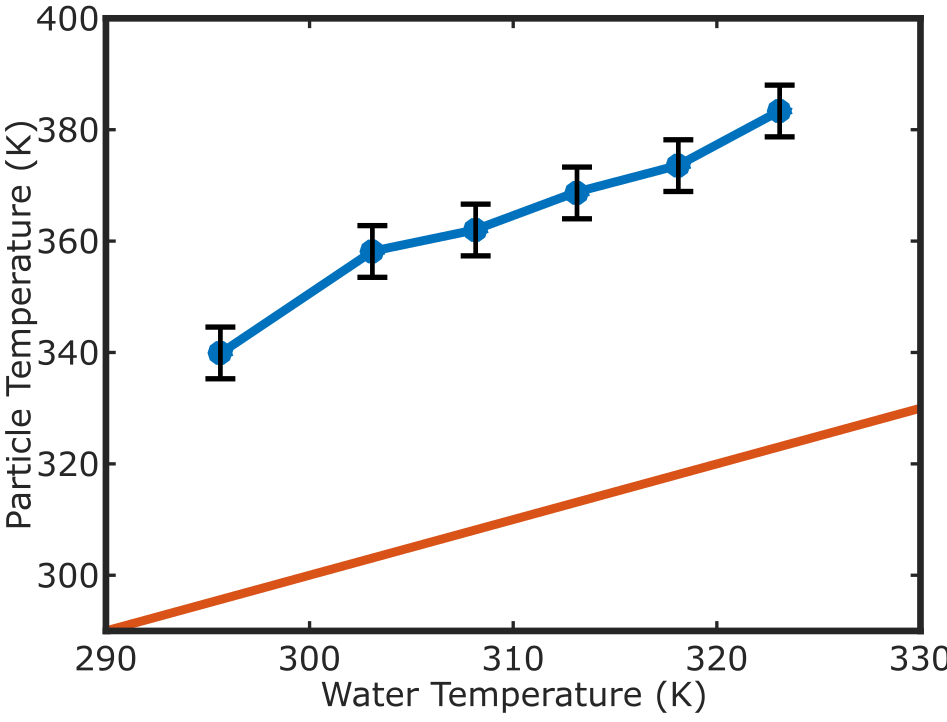
\includegraphics[width=0.50\textwidth]{Chapters/04_Anti-Stokes/Figures/04_Extracted_Temp/04_extracted_temp.png}
\caption{Anti-Stokes emission spectra under $633\nm$ laser excitation at
$510\uW$ but at different temperatures. The inset shows the extracted
temperature as the temperature of the medium increases.}
	\label{fig:AS-temps-rods}
\end{figure}

It is also possible to keep the excitation intensity constant and to vary the
temperature of the surrounding medium. Figure \ref{fig:AS-temps-rods} shows the
extracted temperature from the fitting with equation \ref{eqn:fitting} as a
function of the temperature of the medium. The red line is showing the water
temperature and acts as a guide to the eye. The Figure clearly shows an increase in the extracted temperature while
increasing the temperature of the flow cell. The range of explored
temperatures was from $296\K$ to $320\K$. This range is
enough to observe a change in the anti-Stokes emission spectrum. At higher
temperatures the stability of the setup plays a crucial role in maintaining the
particle in focus during the spectra acquisition time. Longer exposure times and
therefore lower excitation intensities can be employed if particles are actively
maintained in focus.

It would be beneficial therefore to have particles that can withstand higher
excitation powers and that have a well defined plasmon resonance. In this way it
would be possible to use a single wavelength and to reduce the exposure times to
record the spectra. In principle gold nanospheres fulfill these requirements.
They are known to withstand much higher excitation powers without reshaping nor
melting\cite{Hou2015}. Moreover the plasmon resonance of spheres shifts only
slightly with radius, therefore it is possible to predict it using Mie theory
and to eliminate the need of a second laser beam. Sphere samples however
always show a shape distribution that cannot be neglected\cite{Lee2013} and that
induces deviations of the observed resonance from Mie's model.

\begin{figure}[htp] \centering
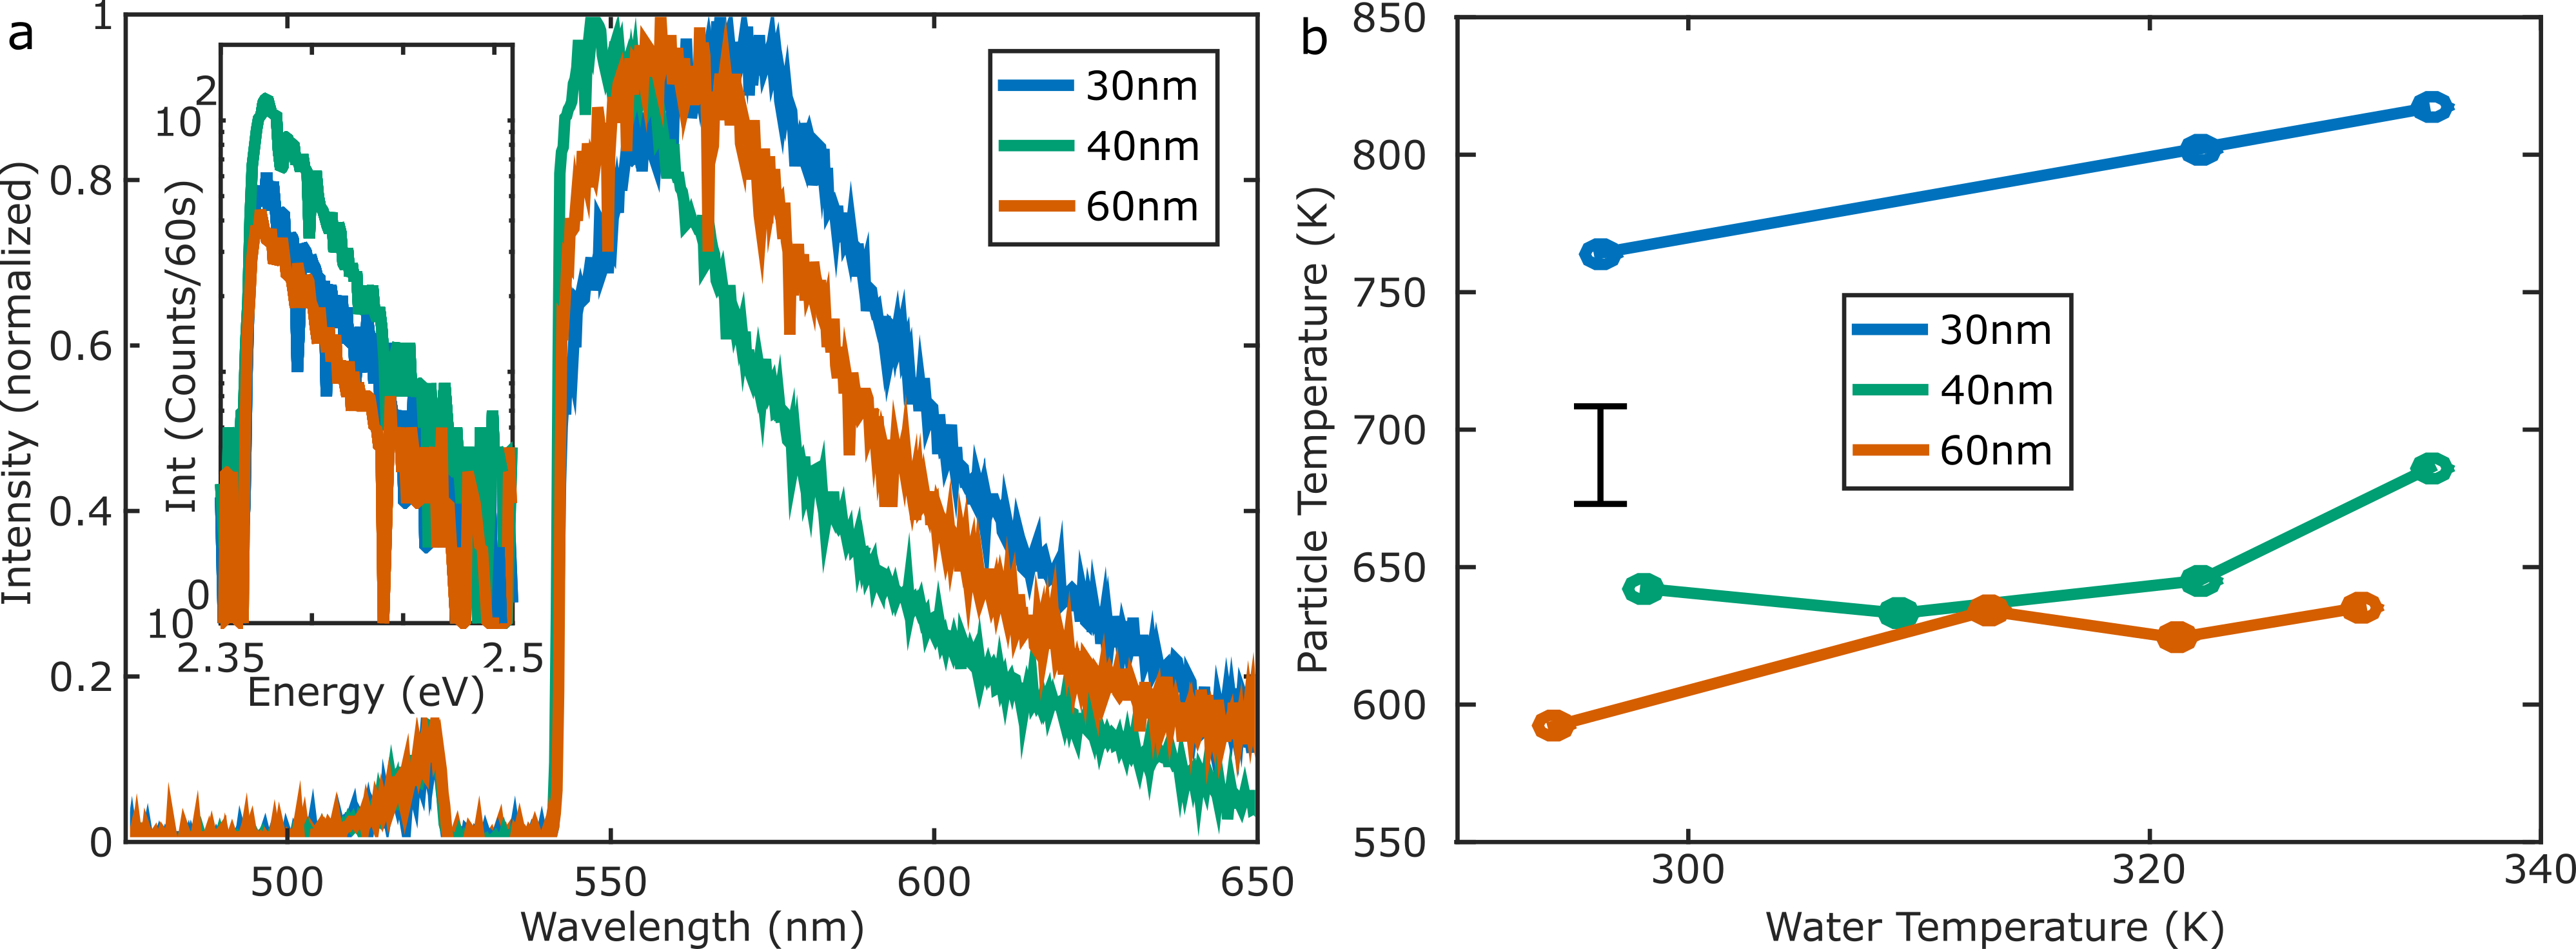
\includegraphics[width=0.90\textwidth]{Chapters/04_Anti-Stokes/Figures/07_Spheres/07_spheres.png}
\caption{Spectra and temperature extraction with spheres of
diameter $60\nm$, $40\nm$ and $30\nm$. a) Normalized luminescence spectra of
three particles under $532\nm$ excitation. The inset shows the detail of the
anti-Stokes emission without normalization. The excitation powers for the three
particles were $1.2\mW$, $2.0\mW$ and $3.6\mW$ respectively. b) Extracted
temperature from these particles while increasing the medium temperature.}
	\label{fig:spheres}
\end{figure}

Figure \ref{fig:spheres}.a shows the normalized luminescence spectra of three
nanospheres of diameters $60\nm$, $40\nm$ and $30\nm$ under $532\nm$ excitation.
As for the nanorods, two very distinctive parts of the spectrum are
distinguishable, the Stokes at longer wavelengths and the anti-Stokes at shorter
ones. From Mie theory it would have been expected a blue shift of the resonance
while diminishing the radius of the particles; however the $30\nm$ sphere seems
to be the most red-shifted. This is most likely due to small anisotropies of the
particles, giving rise to slightly different plasmon resonances. The inset in
Fig.\ref{fig:spheres}.a shows a detail of the anti-Stokes emission for the three
spheres without any further normalization. It has to be pointed out, however,
that the excitation intensities were $1.2\mW$, $2.0\mW$ and $3.6\mW$ to
compensate for the lower cross sections of the smaller particles.

It has to be noted that spheres have not only a smaller cross section than
nanorods of the same volume, but their quantum yield is also one order of
magnitude lower than that of rods\cite{Yorulmaz2012}. The weaker emission from
these particles can be compensated by increasing the excitation power. The
limitation in power it is therefore given by either reaching the melting
temperature of gold or by inducing a phase transition of the surrounding liquid.
The first would induce an irreversible change in shape of the
particles\cite{Zijlstra2009a} the latter would induce a change in the refractive
index of the medium and therefore would induce a shift in the plasmon
resonance\cite{Hou2015}.

Figure \ref{fig:spheres}.b shows the extracted temperature of the three
particles while increasing the medium temperature. It is possible to see that
the small $30\nm$ diameter sphere is $150\K$ hotter than both the $40\nm$ and
$60\nm$. The three curves show an increasing trend, but in this case the
variation of medium temperature amounts to less than $5\%$ the temperature of
the particles. The extracted temperature is several degrees above what would be
expected from the heat equation, considering the absorption cross section given
by Mie theory. An analysis on the error similar to the one performed with rods
yields a relative tolerance of about $5\%$ in the extracted temperature, and
therefore it is not possible to conclude that the increase in the calculated
temperature is in fact given by the increase in the medium's temperature.

The use of spheres would be beneficial for some applications that require higher
excitation powers or smaller particles. The intrinsic heterogeneity of the
samples however, prevents the use of a single wavelength for the
measurements. Ideally white light scattering of the single gold nanospheres
would provide the information on the plasmon resonance needed for the
correct fitting of the anti-Stokes emission.

\section{Conclusions}
Being able to control and monitor temperature at the nanoscale is of utmost
importance in different fields ranging from photothermal therapy\cite{Huang2006}
to nano fabrication\cite{Fedoruk2013}. In this work we have shown a simple
procedure that allows to measure the temperature of single gold nanorods and
nanospheres irradiated under a monochromatic continuous laser and without any
previous calibration. The level of accuracy of the temperature measurement
depends on several factors, but for nanorods it can be estimated to be better
than $6\K$ and for nanospheres around $15\K$.

The model employed for describing the anti-Stokes emission takes into account
the plasmon, responsible for enhancing the emission, as well as Bose-Einstein
statistics to explain the distribution of the excited states of the particles.
It has been shown that the correct characterization of the plasmonic resonance is
fundamental for the proper extraction of temperature, specially in cases
where the excitation wavelength is red-detuned from the resonance.

Particles with a resonance to the red of the excitation wavelength would be more
reliable in the temperature extraction procedure, but would also exhibit a lower
emission towards shorter wavelengths. The trade-off between both effects and
the possibility to fully characterize the plasmon resonance, will determine the
specific particles that are better suited for each application.

In this work we have also explored the possibility of employing gold
nanospheres. Since these particles do not reshape under higher excitation powers
it is possible to compensate their lower cross section by increasing the
irradiation intensity. However, their quantum yield is at least one order of
magnitude smaller than the one of rods, giving an overall lower
photoluminescence intensity. Samples with a narrow shape distribution would be
ideal candidates to temperature extraction since their plasmon can be determined
from Mie theory, avoiding the need of a second excitation source.

We have observed the anti-Stokes emission from particles with three different
diameters. It was already possible to see that the heterogeneity in the shape of
the particles induces plasmon resonances different from the ones predicted from
Mie theory. The variation in the temperature extracted from the anti-Stokes
spectra while increasing the medium's temperature falls within the experimental
error. The obtained temperatures however are much higher than predicted from the
heat equation. The samples normally have a distribution of sizes and shapes,
assuming a perfectly spherical particle leads to an incorrect determination of
the plasmon resonance that propagates into the determination of the surface
temperature. 

The main advantage of the proposed method is that it doesn't require any
calibration, since the only free parameter of the model is the absolute
temperature of the nanoparticle under study. Moreover the recording of the
anti-Stokes spectrum is readily achievable in any confocal microscope with a
coupled spectrometer. A $6\K$ accuracy may suffice for several applications; it
is important to point out that this value can be improved in different ways: by
carefully selecting the particles that show the most favorable plasmon
resonance; by determining the plasmon resonance through white-light scattering,
avoiding the uncertainty in the fit; increasing the exposure times increases the
signal-to-noise ratio; finally an ad-hoc calibration of the temperature can
be performed.

\references{Chapters/04_Anti-Stokes/anti_stokes}

